\documentclass[12pt]{report}
\usepackage{makeidx}
\usepackage{graphicx}
\usepackage{xcolor}
\usepackage{listings}
\usepackage{float}
\usepackage{minted}
\usepackage[left=2cm,right=2cm,top=2cm,bottom=5cm]{geometry}
\textwidth 6in
\textheight 9in
\topmargin 0in
\headsep 0in
\oddsidemargin 0.5cm
\evensidemargin -0.5cm

\lstset{basicstyle=\ttfamily,
  showstringspaces=false,
  commentstyle=\color{red},
  keywordstyle=\color{blue}
}

\title{Skyscrapers Puzzle with\\
Altera FPGA DE1}

\date{\vspace{-5ex}}

\begin{document}
\author{Students: Andrea Giardini - Francesco Venturoli}
\maketitle

\chapter*{Aim of the project}

The project aim is to write a software to run the Skyscrapers puzzle on
a Altera DE1 board \cite{AlteraDE1Board}, allowing users to interact with
it using a keyboard. The final result will be an interactive logic game,
where the user can input digits in the board or ask a suggestion for the
next step. The game needs to recognize when the puzzle is completed and if
the solution provided is correct and respects all the constraints.

\begin{figure}[H]
  \centering
  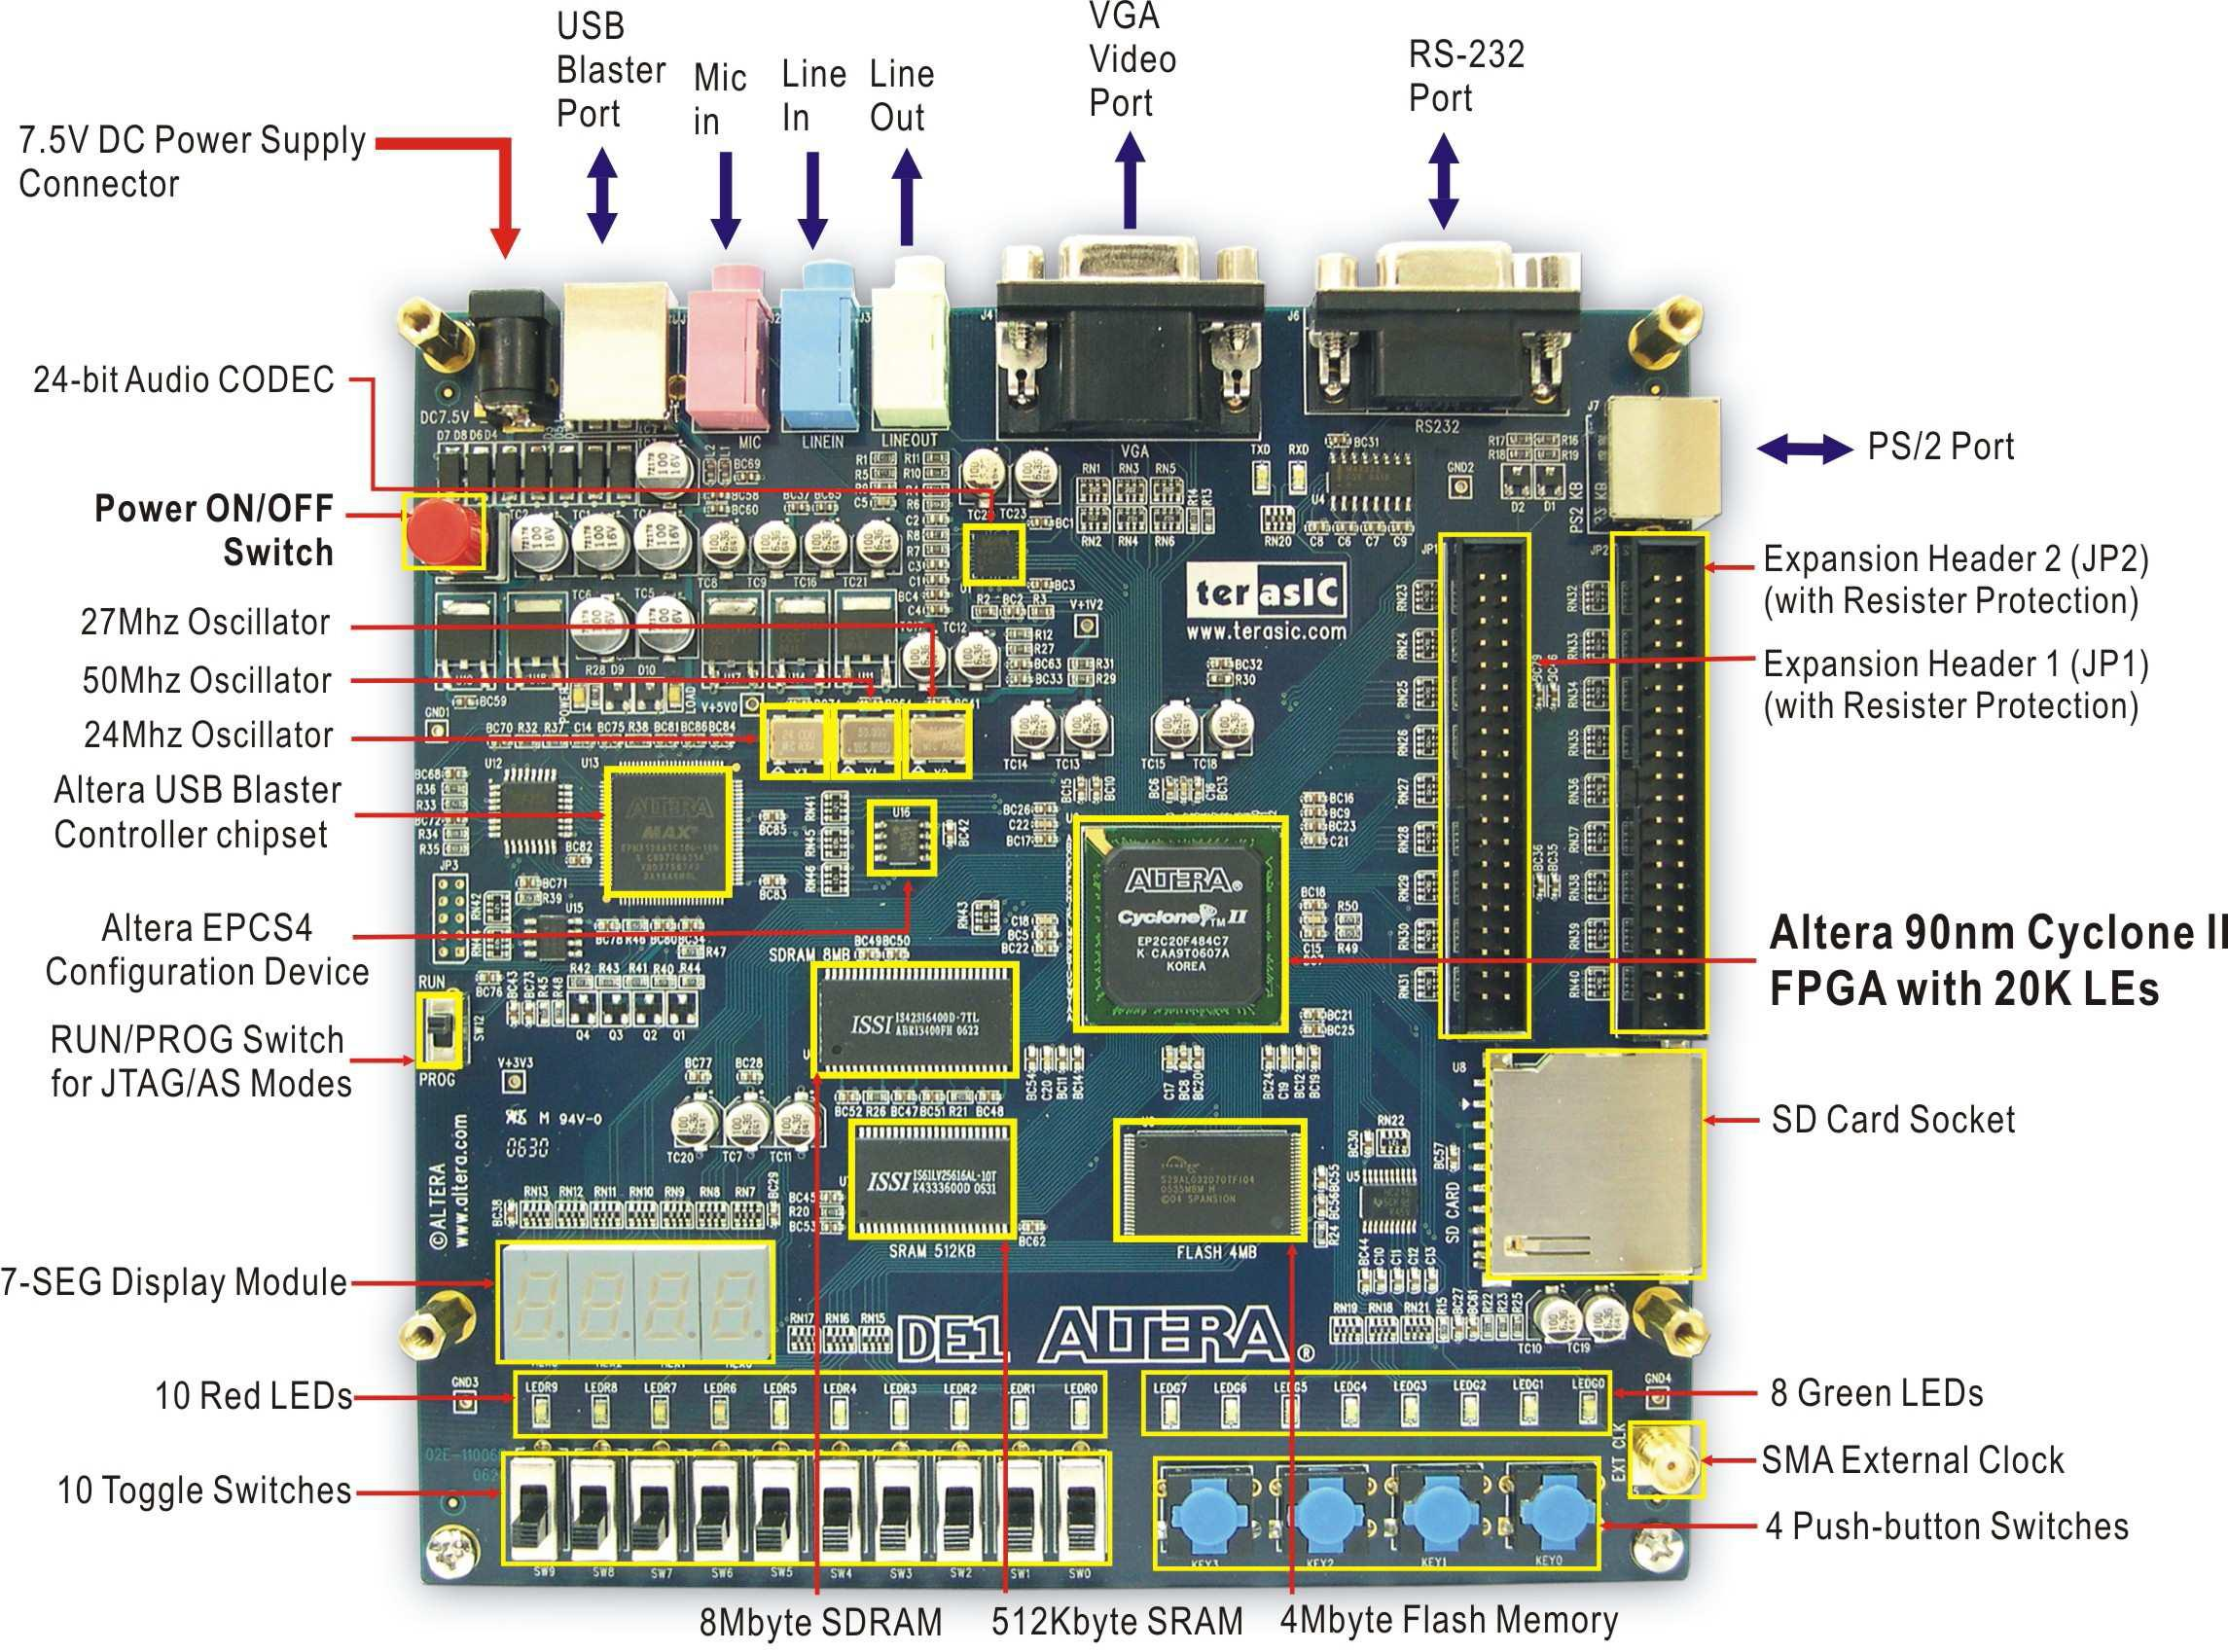
\includegraphics[keepaspectratio,width=0.8\textwidth]{images/Altera_DE1_Board.jpg}
  \caption{Altera DE1 FPGA Board}
\end{figure}

In the proposed game the user needs to be able to move in the game using
the cursors of the keyboard. Entering numbers in the matrix, always using
the keyboard, the user tries to complete the puzzle filling all the blank
spaces with a numeric value. If the user is not able to complete the game
it can solve the board automatically using the algorithms implemented in
the board. Once the puzzle is solved, the board should recognize the
solution and display the winning logo to the user.

\chapter*{Introduction to the puzzle}

Each puzzle consists of an NxN grid with some clues along its sides. The
object is to place a skyscraper in each square, with a height between one
and N, so that no two skyscrapers in a row or column have the same number
of floors. In addition, the number of visible skyscrapers, as viewed from
the direction of each clue, is equal to the value of the clue. Note that
higher skyscrapers block the view of lower skyscrapers located behind
them.

\begin{figure}[H]
  \centering
  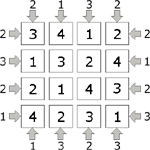
\includegraphics[keepaspectratio]{images/skyscrapers_small_solved.jpg}
  \caption{Solved 4x4 Skyscrapers puzzle}
\end{figure}

There are a number of intuitions that can be addressed immediately,
filling some of the empty spaces with values, others spaces instead need
a combination of more constraints to identify the correct value. The game
can be extended with a bigger matrix or to include parks ( empty spaces, so
buildings with zero height in the matrix ). In our case we decided to
solve the classic version of the puzzle, a 4x4 matrix with no parks.

\chapter*{Game analysis and structure}

To better organize the game we decided to follow the MVC patter, giving to
each class a single responsibility. In the following sections we will
analyse in details what are the responsibilities of each class:

\section*{Control Unit}

The control unit is used in this project to get the inputs from the user
and interpret them. Following that, the interpreted signal is sent to
the Datapath or the View depending on which kind of change we want to
address.

As we specified previously, our intention is to let the user use
a keyboard to play the game. In order to do this we have to read the
serial PS2 line and map the received data with the scan codes of the
keys that we wanted to interpret.

To simplify the problem and keep the Control Unit as clean as possible
we added a new class called \textit{Skyscrapers\_Puzzle\_Keyboard} which is
responsible exclusively to read the data from the keyboard and map it to
scan codes. Using this class we can leave all the logic of translating
the signals to actions to the Control Unit, as it is supposed to be.

The Control Unit has the following signals:

\begin{minted}{vhdl}
  CLOCK        : in  std_logic;
  KEYBOARDDATA : in  std_logic_vector (7 downto 0);
  RESET_N      : in  std_logic;
  TIME_10MS    : in  std_logic;

  CURSOR_POS   : in CURSOR_POS_TYPE;

  -- Connections with DataPath
  MOVE_RIGHT   : out std_logic;
  MOVE_LEFT    : out std_logic;
  MOVE_DOWN    : out std_logic;
  MOVE_UP      : out std_logic;
  NUMBER       : out std_logic_vector (3 downto 0);
  SOLVE        : out std_logic;

  -- Connections with View
  REDRAW     : out   std_logic;
\end{minted}


\section*{Datapath}

\begin{minted}{vhdl}
  CLOCK       : in  std_logic;
  RESET_N     : in  std_logic;
  MOVE_RIGHT  : in  std_logic;
  MOVE_LEFT   : in  std_logic;
  MOVE_DOWN   : in  std_logic;
  MOVE_UP     : in  std_logic;
  SOLVE       : in  std_logic;

  KEYS        : in  std_logic_vector(3 downto 0);

  READY       : out std_logic;
  VICTORY     : out std_logic;
  MATRIX      : out MATRIX_TYPE;
  CONSTRAINTS : out CONSTRAINTS_TYPE;
  CURSOR_POS  : out CURSOR_POS_TYPE;
  WINNER      : out std_logic;
\end{minted}

\section*{View}

\begin{minted}{vhdl}
  CLOCK        : in  std_logic;
  RESET_N      : in  std_logic;

  MATRIX       : in  MATRIX_TYPE;
  CONSTRAINTS  : in  CONSTRAINTS_TYPE;
  CURSOR_POS   : in  CURSOR_POS_TYPE;

  REDRAW       : in  std_logic;

  FB_READY     : in  std_logic;
  FB_CLEAR     : out std_logic;
  FB_DRAW_RECT : out std_logic;
  FB_DRAW_LINE : out std_logic;
  FB_FILL_RECT : out std_logic;
  FB_FLIP      : out std_logic;
  FB_COLOR     : out color_type;
  FB_X0        : out xy_coord_type;
  FB_Y0        : out xy_coord_type;
  FB_X1        : out xy_coord_type;
  FB_Y1        : out xy_coord_type;

  QUERY_CELL   : out block_pos_type;
  CELL_CONTENT : in  board_cell_type;
\end{minted}

\chapter*{Solving algorithm}



\chapter*{Conclusion}


\renewcommand{\bibname}{References}
\begin{thebibliography}{100}

\bibitem{AlteraDE1Board} http://de1.terasic.com/

\end{thebibliography}

\end{document}
